\documentclass[11pt, twoside, a4paper]{book}

\usepackage{graphicx}
\usepackage[utf8]{inputenc}
\usepackage{ngerman}
%\usepackage{lineno}
\usepackage{verbatim}
\usepackage[squaren]{SIunits}
\usepackage{amsmath}
\usepackage{amsfonts}
\usepackage{amssymb}
\usepackage{enumitem}
\usepackage{fancyhdr}
\usepackage{textcomp}
\usepackage{subcaption}
\usepackage[noadjust]{marginnote}
\usepackage{tikz}
\usepackage{nicefrac}
\usepackage{framed}
\usepackage{import}

\usetikzlibrary{calc,intersections}
\usetikzlibrary{arrows}
\usetikzlibrary{decorations.markings}
\usetikzlibrary{decorations.pathreplacing}
\usepackage[european resistors]{circuitikz}
\usepackage[ 
    top=2cm, 
    bottom=2cm, 
    outer=3cm, 
    inner=3cm,
    marginparwidth=2.5cm,
		headheight=14pt
  ]{geometry}

\usepackage{parskip}
\usepackage{pdfpages}

\setlength{\parindent}{0pt}

\newcommand{\experimentheader}[4]
{
  \iftutor{{\bf Schwierigkeitsgrad:} #1\\}
  \iftutor{{\bf Dauer:} #2\\}
  {\bf Ger\"ate:} #3\\
  {\bf Bauteile:} #4
}

\newcommand{\hintboxNone}{0}
\newcommand{\hintboxExclamation}{1}
\newenvironment{hintbox}[4][\hsize]
{
  \def\FrameCommand
  {%
    {\color{#3}\vrule width 3pt}%
    \hspace{0pt}%must no space.
    \fboxsep=\FrameSep\colorbox{#4}%
  }%
  \MakeFramed{\hsize#1\advance\hsize-\width\FrameRestore}%
  \mbox{\textbf{#2}:}%
}
{
  \endMakeFramed
}
\newcommand{\xhintbox}[3]
{
  \begin{hintbox}{Achtung}{red!50}{red!10}
    #3
  \end{hintbox}
}

\newenvironment{hint}
{
  \begin{hintbox}{Hinweis}{green!50}{green!10}
}
{
  \end{hintbox}
}

\newenvironment{definition}
{
  \begin{hintbox}{Definition\\}{white!50}{white!10}
}
{
  \end{hintbox}
}

\newenvironment{important}
{
  \begin{hintbox}{Hinweis}{gray!50}{gray!10}
}
{
  \end{hintbox}
}

\newenvironment{jason}
{
  \begin{hintbox}{Achtung}{red!50}{red!10}
}
{
  \end{hintbox}
}

\newcommand{\mandatoryenumi}
{
  \renewcommand{\labelenumi}{\arabic{enumi}.} 
}
\newcommand{\optionalenumi}
{
  \renewcommand{\labelenumi}{$\bigstar$\quad\arabic{enumi}.} 
}
\newcommand{\mandatoryenumii}
{
  \renewcommand{\labelenumii}{(\alph{enumii})} 
}
\newcommand{\optionalenumii}
{
  \renewcommand{\labelenumii}{$\bigstar$\quad(\alph{enumii})} 
}
\newcommand{\icname}[1]{\mbox{\tt #1}}


  %\newcommand{\iftutor}[1]{}
\newcommand{\ifnotutor}[1]{#1}

  \newcommand{\iftutor}[1]{#1}
\newcommand{\ifnotutor}[1]{}


\newenvironment{tutorhint}{\comment}{\endcomment}
\newenvironment{todo}{\comment}{\endcomment}
\newenvironment{solution}{\comment}{\endcomment}
\iftutor
{
  \renewenvironment{todo}
  {
    \hintbox{Todo}{red!50!yellow!90}{red!50!yellow!20}
  }
  {
    \endhintbox
  }
  \renewenvironment{tutorhint}
  {
    \hintbox{Tutorenhinweis der Stunde}{blue!50}{blue!10}
  }
  {
    \endhintbox
  }
  \renewenvironment{solution}
  {
    \hintbox{L\"osung}{black!80}{black!5}
  }
  {
    \endhintbox
  }
}
\newcommand{\etutorhint}[1]
{
  \iftutor{
    \tutorhint
      #1
    \endtutorhint
  }
}
\newcommand{\esolution}[1]
{
  \iftutor
  {
    \solution
    #1
    \endsolution
  }
}
\newcommand{\etodo}[1]
{
  \iftutor
  {
    \todo
    #1
    \endtodo
  }
}



\begin{document}

\renewcommand{\thechapter}{\arabic{chapter}}
\setcounter{chapter}{2}
\def\chaptername{Versuch}

\chapter{Wechselstrom und R-C-Kreis}
\label{v:15}

In diesem Versuch lernen Sie die Grundlagen der Funktion und Bedienung eines Digital-Speicher-Oszilloskops (DSO), sowie die Auf- und Entladekurve eines Kondensators kennen.

\begin{hint}
	Für diesen Versuch brauchen Sie einen USB Stick, um Bilder vom Oszilloskop abzuspeichern, die Sie für die Auswertung brauchen.\\
	Bitte bringen Sie diesen selbst mit!
\end{hint}

%------------------------------------------------
\section{Stichworte}
%------------------------------------------------

Kathodenstrahl; Braun'sche Röhre; Oszillograph; Ablenkung im elektrischen Feld; Wechselspannung; Kondensator; Kapazität.
%
%------------------------------------------------
\section{Literatur}
%------------------------------------------------

Gehrtsen, Kapitel 7.5.2/3, 8.2.1, 8.2.3
%Teile übernommen aus der Anleitung \textit{''Oszilloskop und Funktionsgenerator''} der Universität Oldenburg
%
%------------------------------------------------
\section{Anwendungsbeispiele}
%------------------------------------------------

R ist die Abkürzung (Symbol) für den elektrischen Widerstand, C für die Kapazität eines Kondensators und L für die Induktivität einer Spule; R-C-Kreise sind Kombinationen aus Widerständen und Kondensatoren, die ein für viele physikalische Vorgänge charakteristisches exponentielles Abklingverhalten zeigen. R-L-Kreise, aus Widerstand und Spule aufgebaut, zeigen auf vereinfachte Weise, was passiert wenn bei den meisten Haushaltsgeräten die Spannung eingeschaltet wird (z. Bsp. Glühbirnen).\\

Eine Zellmembran mit geringer Leitfähigkeit als Grenzschicht zwischen gut leitenden elektrolytischen Flüssigkeiten stellt eine elektrische Parallelschaltung eines Widerstandes (Membranwiderstand) und eines Kondensators (Membrankapazität) dar. Aus der Anwendung entsprechender physikalischer Modellvorstellungen kann ein Verständnis der physiologischen Vorgänge und Messtechniken zur Untersuchung von Zelleigenschaften und interzellulären Vorgängen gewonnen werden.

%------------------------------------------------
\section{Theoretischer Hintergrund}
%------------------------------------------------

\subsection{Oszilloskop} \label{chap:Oszilloskop}

\begin{figure}[hb]
	\centering
		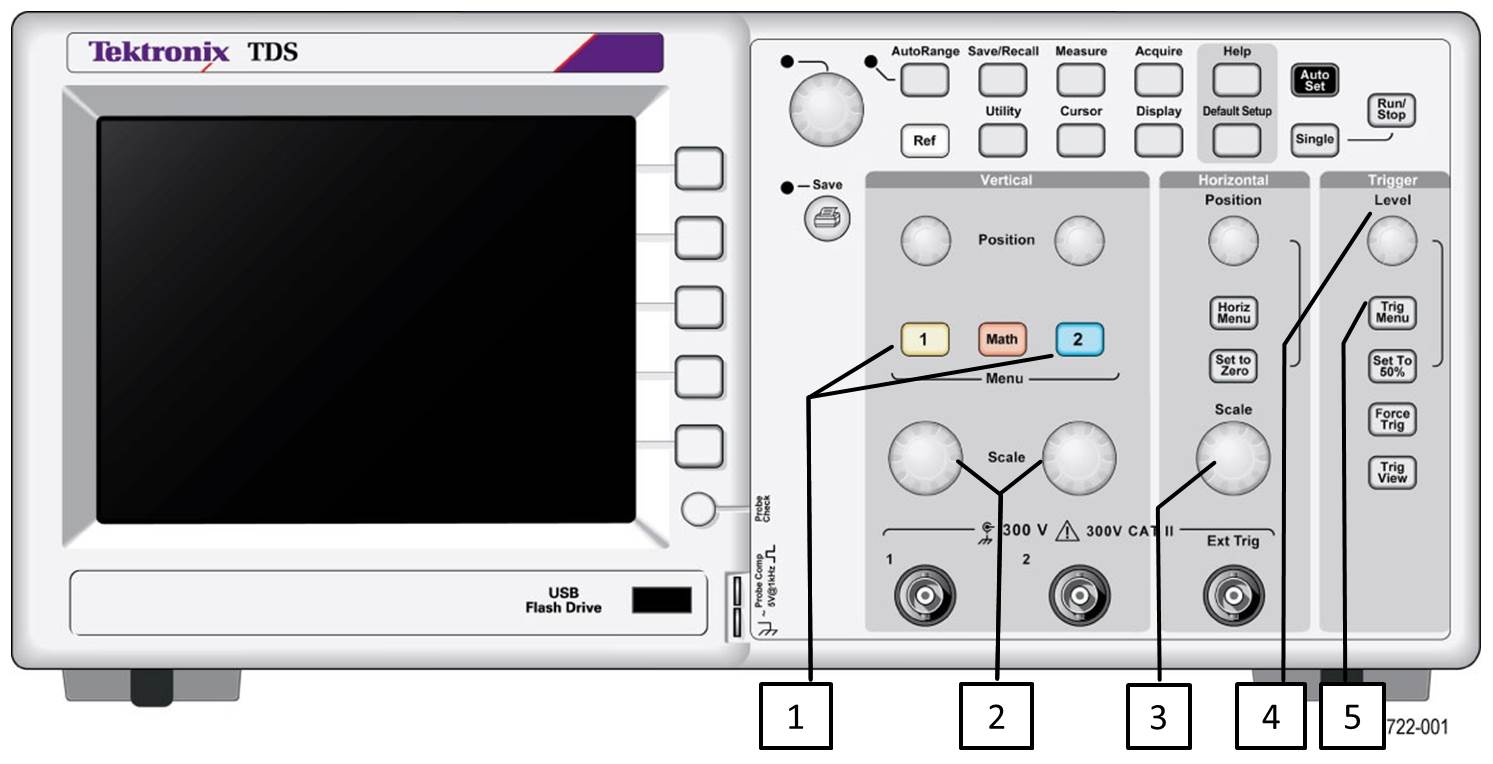
\includegraphics[width=0.5\textwidth]{Abbildungen/TDS2000.JPG}
	\caption{Front des TDS 2001C.}
	\label{fig:TDS2000}
\end{figure}

Will man schnell laufende Vorgänge, z.B. Wechselspannungen oder Impulse, stetig messen und in Abhängigkeit von der Zeit registrieren, so verwendet man ein Oszilloskop. Dieses stellt Spannungen direkt als Funktion der Zeit dar und ermöglicht so die Beobachtung von Vorgängen mit hoher Frequenz.

  Meist benutzt man das Oszilloskop im sogenannten \textit{YT-Modus}, bei dem auf der horizontalen X-Achse des Displays die Zeit $t$ dargestellt wird. Die \textit{Zeitbasis}, d.h. die Skalierung der Zeitachse, kann durch den horizontalen Wahlschalter zwischen \unit{5}{\nano\second} pro Kästchen und \unit{50}{\second} pro Kästchen einstellen. 
  Die Kästchen werden am Oszilloskop als DIV (für Division) bezeichnet. 
  Weitere Eigenschaften der Zeitachse können in dem Menü eingestellt werden, welches nach Drücken der 
  Taste HORIZ MENU angezeigt wird. Für die richtige Wahl der Zeitbasis sollten Sie sich klar machen, mit welcher Frequenz die Spannung am Eingang des Oszilloskops sich verändert.

  Auf der vertikalen Y-Achse wird die am Eingang gemessene Spannung dargestellt. Die Skala der Y-Achse kann über den vertikalen Wahlschalter für jeden der vier Kanäle des Oszilloskops getrennt zwischen \unit{20}{\milli\volt} pro Kästchen und \unit{50}{\volt} pro Kästchen eingestellt werden. Zur richtigen Wahl des Y-Verstärkungsfaktors sollten Sie sich klarmachen, welche Spannung Sie an der zu messenden Stelle Ihrer Schaltung erwarten. 

  \paragraph{Kanaleigenschaften}
  Weitere Eigenschaften der Y-Achse können im sogenannten \textit{Kanalmenü} eingestellt werden, welches nach Drücken der Taste CH MENU für den entsprechenden Kanal angezeigt wird. Diese Eigenschaften können für die beiden Kanäle unabhängig von einander eingestellt werden. 
  \begin{itemize}
    \item KOPPLUNG: Es ist möglich, über eine zum Eingang in Reihe geschaltete Kapazität, den Gleichspannungsanteil der Eingangsspannung zu unterdrücken. Dies geschieht, wenn die Kopplung des Kanals auf AC gestellt wird. Dieser Modus ist nützlich, um Spannungsänderungen zu untersuchen und beschleunigt die Arbeit mit dem Oszilloskop erheblich,
      falls der Gleichspannungsanteil tatsächlich irrelevant ist.
      \begin{hint}
        Während des Versuchs stellen Sie die Kopplung bitte auf DC.
      \end{hint}

    \item BANDBREITE: Die Bandbreiteneinstellung bestimmt die frequenzabhängig Unterdrückung von Eingangssignalen. Wenn Sie Signale in der Größenordnung MHz darstellen wollen, sollten Sie darauf achten, dass die Bandbreite auf den maximalen Wert für den Oszilloskoptyp eingestellt ist, da ansonsten die Signalform stark verzerrt dargestellt wird.
    \item TASTKOPF: Die Tastköpfe, mit denen Sie Ihre Schaltung untersuchen, können die Eingangsspannung über einen einstellbaren Spannungsteiler um den Faktor 10 unterdrücken. Dies dient dazu, größere Spannungen auf dem Oszilloskop darstellen zu können, als man sicher an den Eingang anschließen könnte ohne Bauteile im Oszilloskop zu zerstören. 
    Stellen Sie sicher, dass die Unterdrückung des Tastkopfes und die im Kanalmenü eingestellte Unterdrückung übereinstimmen, da Sie ansonsten andere Spannungswerte am Oszilloskop ablesen, als wirklich in der Schaltung anliegen.
			\begin{hint}
				Im Versuch stellen Sie bitte sicher, dass keine Unterdrückung (1X) eingestellt ist und dass Spannung gemessen wird und nicht Strom.
			\end{hint}
    \item INVERTIERUNG: Hiermit können Sie anstelle der Spannung $U$ die invertierte Spannung $-U$ auf dem Oszilloskop darstellen. 
			\begin{hint}
				Im Versuch stellen Sie bitte sicher, dass keine Invertierung eingestellt ist.
			\end{hint}
  \end{itemize}

  \paragraph{Trigger} 
  Das Oszilloskop stellt die Eingangsspannung auf dem Display dar, wenn die sogenannte \textit{Triggerbedingung} erfüllt ist. Diese stellt man im Trigger Menü ein, welches nach Drücken der Taste TRIG MENU angezeigt wird. 
  Das Oszilloskop stellt mehrere verschiedene Arten von Triggerbedingungen zur Verfügung. So kann unter anderem auf Pulse bestimmter Breite getriggert werden. Im Praktikum ist allerdings der meistbenutzte Triggertyp der sogenannte \textit{Flankentrigger}. Eine typische Triggerbedinung lautet: Triggere, wenn die Spannung am Kanal 1 einen Wert von \unit{0.1}{\volt} überschreitet.\\
  Diese Bedingung besteht aus drei separat einstellbaren Teilen:
  \begin{enumerate}
    \item Die Triggerquelle, d.h. die Spannung welches Kanals soll betrachtet werden? Wird im Triggermenü über den Punkt QUELLE eingestellt.
    \item Der Triggertyp, d.h. Eingangsspannung soll den Schwellenwert von unten überschreiten (positive oder steigende Flanke) oder von oben unterschreiten (negative oder fallende Flanke). Wird im Triggermenü über den Punkt FLANKE eingestellt.
    \item Der Schwellenwert, d.h. wie groß ist die Spannung, mit der die Engangsspannung verglichen werden soll? Wird über den Drehknopf LEVEL eingestellt.
  \end{enumerate}
  Eine weitere wichtige Eigenschaft des Triggers ist der \textit{Triggermodus} (Triggermenü, Punkt MODUS):
  \begin{itemize}
    \item Triggermodus AUTO: Das Display wird in regelmäßigen Abständen neu aufgebaut, unabhängig davon, ob die Triggerbedingung erfüllt ist. Dieser Modus eignet sich dafür, eine erste Vorstellung des Signals zu bekommen, während noch kein korrekter Trigger eingestellt ist.
    \item Triggermodus NORMAL: Das Display wird nur dann neu aufgebaut, wenn die Triggerbedingung erfüllt ist. Dieser Modus eignet sich, um schnelle Veränderungen der Eingangsspannung, wie zum Beispiel logische Signale, zu untersuchen.
      Ist die Triggerbedingung in kurzen Abständen verlässlich erfüllt,
      verhalten sich NORMAL und AUTO identisch. Sie können also häufig im
      Modus AUTO verbleiben und nur zu NORMAL wechseln, wenn zwischen
      zwei Triggern zu viel Zeit vergeht.
    \item
      Triggermodus STOP: Das Oszilloskop beh\"alt die letzte Aufnahme.
    \item
      Triggermodus SINGLE: Falls Sie eine funktionierende Triggerbedingung haben
      und sich eine einzige Aufnahme des Eingangssignals anschauen m\"ochten,
      k\"onnen Sie auf SINGLE wechseln. Das Oszilloskop wartet dann auf eine
      Triggerbedingung, nimmt genau eine Aufnahme auf und wechselt zu STOP.
  \end{itemize}
	
\subsubsection{Betrieb}

Da wir nur auf Pos. I messen, wird der Tastkopf bei CH 1 eingesteckt, die zugehörige Massenverbindung erfolgt an der Bananenbuchse daneben.\\
Mit dem Drehknopf (2) wird die Empfindlichkeit der Y-Achse eingestellt: Stellung 2~V bedeutet, dass jedes Kästchen auf dem Bildschirm 2~V hoch ist.\\

\noindent
Alle Oszilloskope (dieser Welt ?) werden nach diesem Schema bedient. Die vielen Knöpfe verführen zum Spielen, und wir möchten alle ermutigen, zu probieren, was die einzelnen Schalter bewirken. Diese Anleitung führt - hoffentlich - wieder zu einer Schalterstellung zurück, die eine richtige Messung ermöglicht.

\subsection{Wechselspannung und Wechselstrom}

Als Wechselspannung bezeichnet man eine periodische Spannung mit sinus- oder kosinusförmigem Verlauf:
\begin{equation}
 U(t) = U_0 \sin\omega t
\end{equation}
%
Die Wechselspannung verursacht an einem Bauteil einen Wechselstrom, der eine zeitliche Versetzung $t'$ (Phasenverschiebung $\delta$) gegenüber der Spannung haben kann:
\begin{equation}
 I(t) = I_0 \sin\omega(t-t') = I_0 \sin(\omega t - \delta)
\end{equation}

\noindent
Wechselspannungen werden technisch meist durch Induktion erzeugt (Dynamogenerator). Wird eine Leiterschleife mit konstanter Winkelgeschwindigkeit in einem homogenen Magnetfeld gedreht, so wird in dieser auf Grund des Induktionsgesetzes eine Wechselspannung induziert.\\

\noindent
In Wechselstromkreisen gibt es unterschiedliche Angaben zur Charakterisierung der Größe von Spannung und Strom: die Amplituden oder Scheitelwerte ($U_0$, $I_0$), die Effektivwerte ($U_{eff}$, $I_{eff}$) und die Spitze-Spitze-Werte ($U_{SS}$):
\begin{itemize}
 %
 \item \underline{Amplitude (Scheitelwert):} Die Amplituden geben die Maxima von Spannung oder Strom an; sie entsprechen dem Amplitudenbegriff der trigonometrischen Funktionen.
 %
 \item \underline{Effektivwert:} Die Effektivwerte von Spannung und Strom sind charakteristische Werte, deren Produkt (wie im Fall des Gleichstroms) die (mittlere) joulesche Wärmeleistung ergibt:
  \begin{equation}
   \bar{P} = U_{eff}\, I_{eff} = \frac{U_0}{\sqrt{2}}\,\frac{I_0}{\sqrt{2}}
  \end{equation}
	\begin{hint}
		Berechnet wird der Effektivwert, z.Bsp. der Spannung, als 
		\begin{equation*}
			U_{eff} = \sqrt{\frac{1}{T} \int_{t_0}^{t_0 +T}{u^2 du}} = \sqrt{\bar{u^2}}
		\end{equation*}
		Für eine sinusförmige Wechselspannung $u=u_0 sin(\omega t)$ ergibt sich
		\begin{equation*}
			\bar{u^2} = u_0^2 \bar{sin^2(\omega t)} = u_0^2\frac{1}{2}
		\end{equation*}
		Somit ergibt sich für den Effektivwert der Spannung
		\begin{equation} \label{eq:Effektivspannung}
			U_{eff} = \sqrt{\bar{u^2}} = \frac{u_0}{\sqrt{2}}
		\end{equation}
	\end{hint}
 %
 \item \underline{Spitze-Spitze-Wert:} In besonderen Fällen wird für Spannungen die Differenz zwischen größtem und kleinstem Wert als sogenannter Spitze-Spitze-Wert $U_{SS}$ angegeben.
 %
\end{itemize}

Die Amplituden und $U_{SS}$ können auf dem Oszilloskop direkt beobachtet werden. Die Effektivwerte werden mit Multimetern gemessen, die für Wechselspannungen und -ströme einen eingebauten Gleichrichter enthalten und für diese Messbereiche in Effektivwerten kalibriert sind.\\

Analog zum ohmschen Widerstand R wird als Wechselstromwiderstand Z (Scheinwiderstand oder Impedanz) das Verhältnis der Amplituden von Spannung und Strom definiert:
\begin{equation}
 Z = \frac{U_0}{I_0} = \frac{U_{eff}}{I_{eff}}
 \label{eq:Z}
\end{equation}
Bei ohmschen Widerständen stimmen Gleich- und Wechselstromwiderstand überein. Bei anderen Bauteilen, wie Kondensatoren und Spulen, ist dies nicht der Fall.

\subsection{Kondensator und R-C-Kreis}

Ein Kondensator ist ein Speicher für elektrische Ladung. Die in einem Kondensator befindliche Ladung $Q$ ($Q$ auf der einen Platte und $-Q$ auf der anderen) ist proportional zur ''Größe'' des Kondensators (Kapazität $C$) und zur Spannung $U$ (die Kapazität $C$ ist definiert als Verhältnis von Ladung zu Spannung):
\begin{equation}
 Q = C\cdot U
 \label{eq:Q}
\end{equation}

\noindent
Die Einheit der Kapazität ist:
\begin{equation}
 \mathrm{\left[C\right] = 1\frac{As}{V} = 1 F \quad (Farad)}
\end{equation}

\noindent
Der Strom $I_C$ durch den Kondensator ist die zeitliche Ableitung der Ladung, mit Gleichung (\ref{eq:Q}):
\begin{equation}
 I_C = \frac{dQ_C}{dt} = C\,\frac{dU_C}{dt}\; .
 \label{eq:I_C}
\end{equation}
Wie man sieht ist der Strom groß, wenn sich die Spannung schnell ändert.\\
Stellt man diese Gleichung nach der Spannung frei
\begin{equation}
 U_C = \frac{1}{C}\int{I_C\, dt}
\end{equation}
so sieht man, dass sich die Spannung beim Aufladen eines Kondensators verhält wie das Integral über den Strom.

Nun werde ein (geladener) Kondensator der Kapazität $C$ mit einem Widerstand $R$ zu einem geschlossenen Stromkreis verschaltet.
\begin{figure}[h]
	\centering
		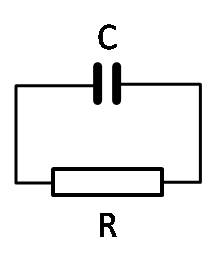
\includegraphics[width=.1\textwidth]{Abbildungen/RC-Kreis.jpg}
	\caption{R-C-Kreis}
	\label{fig:RC-Kreis}
\end{figure}
Die Spannung am Kondensator ($U_C$) ergibt sich aus Gleichung (\ref{eq:I_C}), die Spannung am Widerstand aus der Definition
\begin{equation}
 U_R = R\, I_R\; .
\end{equation}
Nach der Maschenregel muss die Summe aller Ströme in der Masche Null sein. Mit $I = I_C = I_R$ folgt:
\begin{equation}
 U_C + U_R = \frac{1}{C}\int{I\, dt} + R I = 0\; .
\end{equation}
Durch Ableitung nach der Zeit erhält man eine Differentialgleichung für den Strom als Funktion der Zeit:
\begin{equation}
 \frac{dI}{dt} + \frac{1}{RC}\,I = 0\; .
\end{equation}
Diese Differentialgleichung wird gelöst durch die Funktion
\begin{equation}
 I(t) = I_0\, e^{-t/RC}
 \label{eq:Entladekurve}
\end{equation}
Beim Entladen entwickelt sich ein exponentiell mit der Zeit abklingender Strom (ebenso beim Aufladen). Das Produkt $RC$ im Exponenten von Gleichung (\ref{eq:Entladekurve}) bestimmt quantitativ die Abnahme des Stromes und wird als Zeitkonstante bezeichnet.\\

Betrachten wir nun den Wechselstromwiderstand des Kondensators.\\
Mit einer Wechselspannung der Form $U(t) =  U_0\cos\omega t$ finden wir den Strom durch den Kondensator gemäß Gleichung (\ref{eq:I_C}). Mit der Definition des Wechselstromwiderstandes (Gleichung (\ref{eq:Z}) ) berechnet man die Impedanz des Kondensators zu:
\begin{equation}
 Z_C = \frac{U_0}{I_0} = \frac{1}{\omega\, C}\; .
\end{equation}
Ursache des Widerstandes ist die sich aufbauende Gegenspannung am Kondensator. Die dabei umgesetzte Energie bleibt jedoch als elektrische Feldenergie im Kondensator gespeichert und wird während der Entladephase an den Kreis zurückgegeben. Ein (idealer) Kondensator setzt dem Strom einen Widerstand entgegen, der ohne Energieabgabe nach außen bleibt und deshalb als Blindwiderstand bezeichnet wird.\\

Wegen der Frequenzabhängigkeit des Wechselstromwiderstandes von Kondensatoren (und von Spulen) können mit diesen Bauteilen sogenannte Filter gebaut werden, die aus einem Wechselspannungsspektrum bestimmte Frequenzbereiche heraussieben. Solche Filter werden oft benötigt, um in elektrischen Mess- und Steuerkreisen die interessierenden Signale auszuwählen und Störsignale mit anderen Frequenzen abzutrennen. \\
Ein einfaches Beispiel ist die Reihenschaltung eines Kondensators mit einem Widerstand als Spannungsteiler:
\begin{figure}[ht]
	\centering
		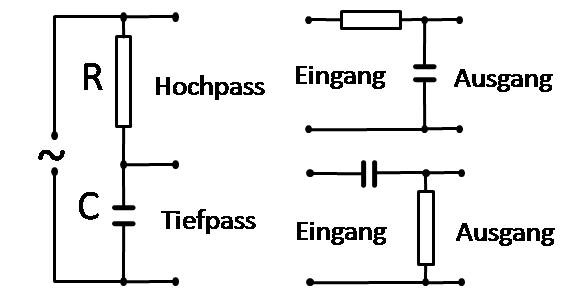
\includegraphics[width=0.5\textwidth]{Abbildungen/Paesse_gross.jpg}
	\caption{Hoch- und Tiefpassschaltungen}
	\label{fig:Hoch-Tiefpass}
\end{figure}
Eine Teilspannung ist proportional dem Teilwiderstand, über dem sie abgegriffen wird. Für tiefe Frequenzen ist der Widerstand des Kondensators groß, so dass hier der Hauptanteil der Eingangsspannung abfällt. Der Abgriff über dem Kondensator stellt einen \textit{Tiefpass} dar. Für hohe Frequenzen ist umgekehrt der Widerstand des Kondensators klein und der des Widerstandes vergleichsweise groß, so dass der Abgriff über dem Widerstand als \textit{Hochpass} wirkt.
%------------------------------------------------
\section{Fragen zur Vorbereitung}
%------------------------------------------------

\begin{enumerate}
 %
 \item Was ist eine Wechselspannung? Wie kann man sie mathematisch beschreiben (Beispiel)? 
		\begin{solution}
			Wechselspannung ist eine zeitlich nicht konstante Spannung, die jedoch meistens einen periodischen Verlauf hat und bei der sich typischerweise im Laufe der Zeit das Vorzeichen ändert. Sie kann meist durch einen sinusförmigen Verlauf beschrieben werden, z.Bsp.
			\begin{equation*}
				U(t) = U_0 \sin\omega t
			\end{equation*}
		\end{solution}
 %
 \item Was versteht man unter der Schwingungsdauer/Periode einer Wechselspannung? Wie lautet der Zusammenhang zwischen Periode und Frequenz?
		\begin{solution}
			Schwingungsdauer $T$ ist die Zeit zwischen zwei gleichen Schwingungszuständen der Spannung. Für die Frequenz gilt: $$f = \frac{\omega}{2\pi} = \frac{1}{2\pi T}$$.
		\end{solution}
 %
 \item Was versteht man unter einer Effektivspannung/einem Effektivstrom? Wie lautet der entsprechende Zusammenhang für eine sinusförmige Wechselspannung?
		\begin{solution}
			Der Effektivwert, z.Bsp. die Effektivspannung, einer zeitlich veränderlichen Größe ist diejenige Gleichgröße, also Betrag einer Gleichspannung, die in einem ohmschen Widerstand im zeitlich konstanten Mittel dieselbe Leistung (Wärme pro Zeitspanne) umsetzt. Zur Berechnung siehe \ref{eq:Effektivspannung}.
		\end{solution}
 %
 \item Was ist ein Kondensator? Wie sieht ein Plattenkondensator aus?
		\begin{solution}
			Ein Kondensator besteht aus zwei Elektroden beliebiger Geometrie (Platten-, Zylinder-, sphärischer Kondensator), welche durch ein Dielektrikum voneinander getrennt sind. Bei einem idealen Kondensator besteht kein ohmscher Kontakt, i.e. $R=\infty$. Die negative Elektrode wird mit Elektronen aufgeladen, so werden auf der anderen positive Ladungen induziert. Ändert sich die Ladung über die Zeit, so scheint es, als würde Strom durch die Kapazität fließen.\\
			Ein typischer Plattenkondensator besteht aus zwei parallelen Platten, die so große angenommen werden, dass Effekte an ihren Rändern vernachlässigt werden können. Zwischen den Platten befindet sich Luft oder ein anderes Dielektrikum mit hohem spez. Widerstand.
		\end{solution}
 %
 \item Was ist die Kapazität eines Kondensators? Wie hängt sie mit Ladung und Spannung zusammen?
		\begin{solution}
			Die Kapazität beschreibt, wie groß das elektrische Feld zwischen den Elektroden, i.e. die Spannung über den Kondensator, ist bei Beladung der Elektroden mit einer bestimmten Ladung. D.h. dass die Kapazität eine Eigenschaft des Kondensators ist.
			\begin{equation*}
				Q = C\cdot U\quad,
			\end{equation*}
			mit der Ladung $Q$, der Spannung über den Kondensator $U$ und seiner Kapazität $C$.
		\end{solution}
 %
 \item Beschreiben Sie anhand einer kleinen Skizze (Spannung in Abhängigkeit der Zeit) die Auf- und die Entladung eines Kondensators über einen ohmschen Widerstand! Wie hängt die Auf-/Entladung des Kondensators von der Größe des Widerstandes ab?
 %
% \item Was ist eine Braun'sche Röhre (Skizze und kurze Erklärung)? Stichworte: Wie wird der Elektronenstrahl erzeugt? Wie wird er abgelenkt?
 %
 \item Wozu dient ein Oszilloskop?
	\begin{solution}
		Dazu, zeitlich veränderliche Spannungen visuell darzustellen.
	\end{solution}
 %
 \item Wozu dient der Trigger bei einem Oszilloskop? Wie ist eine typische Triggerbedingung definiert?
	\begin{solution}
		Trigger dient dazu, interessante Spannungsänderungen im Display darzustellen (egal ob periodische Änderung oder einzelne Pulse). \\
		Eine typische Triggerbedingung lautet: Triggere wenn Eingangsspannung die Trigger- oder Kippspannung unter-/überschreitet.
	\end{solution}
 %
\end{enumerate}

%------------------------------------------------
\section{Durchführung} 
%------------------------------------------------

\begin{enumerate}
 \item Bevor Sie mit dem Versuch beginnen, lesen Sie Kapitel \ref{chap:Oszilloskop} noch einmal durch, um sich mit der Bedienung des Oszilloskops vertraut zu machen.
 %
 \item In diesem ersten Versuchsteil sollen Sie sich mit dem Oszilloskop vertraut machen. Stellen Sie eine sinusförmige Wechselspannung auf dem Bildschirm des Oszilloskops dar und beobachten die Abbildung bei verschiedenen Einstellungen des Oszilloskops.\\
  (Anmerkung: In diesem Versuchsteil werden keine für die Auswertung relevanten Messungen durchgeführt.)\\
  
  \noindent
  %Einschalten des Oszilloskops (1), Regeln von Helligkeit (18) und Schärfe (20). Man vergewissere sich, dass folgende Schalter im oberen Bedienungsfeld die richtige Position haben (sie werden nicht 
  %gebraucht!): TV Set: off; Delay: off; Hold-off: rechter Anschlag; Trig: AT.\\
	Man wähle den größten Messbereich für die Eingangsspannung (2). Man verbinde den Eingang des Oszilloskops mit dem Ausgang des Netzgeräts mit Hilfe des Anschlusskabels und einer Massenleitung. Man
	verändere die Zeitauflösung (3) und den Trigger-Level (4) und beobachte das Bild auf dem Bildschirm. Man ändere die Polarität der Triggerflanke (Trig Menu). Man ändere die Ablenkempfindlichkeit (2). Überzeugen Sie sich davon, dass eine Änderung der Ablenkempfindlichkeit bzw. der Zeitauflösung zwar die Auflösung ändert, nicht aber die Spannungsamplitude (in Volt) bzw. die Periode (in Sekunden) der Wechselspannung.
 %
 \item Messen Sie mit Hilfe des Vielfachmessgerätes die Werte der Widerstände $R_C$ und $R_L$ in der Versuchsbox ''Wechselspannungsversuch''. Dazu verbinden Sie die Ausgänge des Vielfachmessgerätes mit 
 	den Anschlussbuchsen ober- und unterhalb des Widerstandes $R_C$ (bzw. $R_L$). Legen Sie keine äußere Spannung an! Diese verfälscht die Messung und kann das Vielfachmessgerät beschädigen.\\
  Bitte notieren Sie die Nummer der Versuchsbox. Anmerkung: Der Widerstand $R_L$ (und die Nummer der Versuchsbox dienen lediglich dem Assistenten als Referenz und werden in der Auswertung nicht 
  benötigt).
 %
	
	\begin{figure}[t]
		\centering
			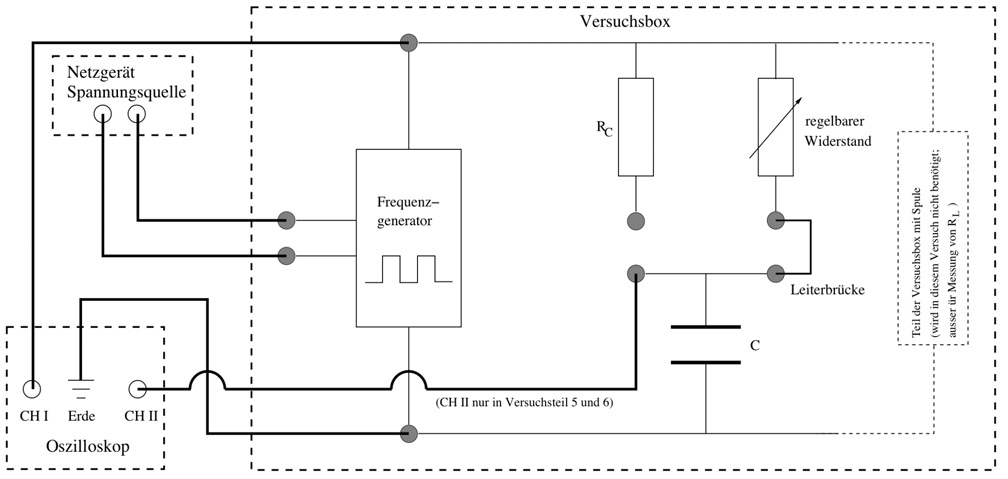
\includegraphics[width=\textwidth]{Abbildungen/Schaltung.jpg}
		\caption{Schaltskizze für den weiteren Versuchsverlauf.}
		\label{fig:Schaltung}
	\end{figure}
	
 \item Verbinden Sie das Netzteil mit dem Eingang des Frequenzgenerators. Stellen Sie dabei sicher, dass die Ausgangsspannung des Netzteils eine Amplitude von 24~V hat.\\
	\begin{minipage}{0.45\textwidth}
		Verbinden Sie das Oszilloskop mit dem Ausgang des Frequenzgenerators. Die Ausgangsspannung des Frequenzgenerators wird auf dem Bildschirm dargestellt (siehe Abbildung \ref{fig:Schaltung}). Messen Sie die Maximalamplitude 
		$U_0$ sowie die Schwingungsdauer und die Frequenz des Ausgangssignals. Schätzen Sie jeweils Ihre Ablesefehler ab.
	\end{minipage} 
	\hfill
	%
	\begin{minipage}{0.45\textwidth}
		\raggedright
			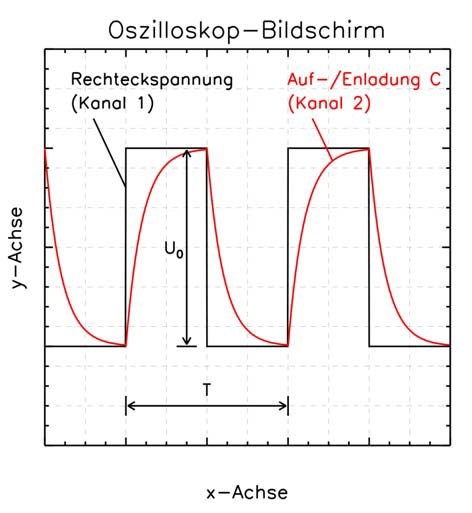
\includegraphics[width=0.7\textwidth]{Abbildungen/Oszi.jpg}
			\label{fig:Oszi}
	\end{minipage}
 %
 \etutorhint{Das Ausgangssignal des Funktionsgenerators sollte Rechteck-förmig sein und eine Frequenz von etwa 10~kHz haben. Wenn die Praktikanten das Signal nicht finden können, bitte zunächst die Zeitbasis des Oszilloskops überprüfen.}
%
 \etutorhint{Nur eine Erdverbindung zwischen Oszi und Frequenzgenerator nötig, da die Außenleiter der beiden Kanäle des Oszilloskops miteinander verbunden sind.}
 %
\begin{hint}
	Stecken Sie für die nächsten Messungen den mitgebrachten USB Stick in den vorderen USB Anschluß des Oszilloskops. Daraufhin sollte eine kurze Meldung erscheinen, dass der Stick erkannt wurde. Nun können Sie durch Druck auf die Taste ''Drucken'' den momentanen Bidschirminhalt des Oszilloskops als jpg-Datei speichern. Notieren Sie sich, welche Datei bei welchen Messbedingungen aufgenommen wurde, da das Oszilloskop die Dateien nur mit einer laufenden Nummer unterscheidet.
	\etutorhint{Wenn ein mitgebrachter USB Stick nicht erkannt wird, können die Tutoren einen der vorhandenen USB Sticks ausgeben. Bitte notieren und der Person nur das Testat erteilen, wenn der Stick zurückgegeben wurde.}
\end{hint}

 \item Auf- und Entladung eines Kondensators über einen Widerstand:\\
	Verbinden Sie den regelbaren Widerstand über die Leiterbrücke mit dem Kondensator. Messen Sie nun mit dem zweiten Kanal des Oszilloskops den Spannungsabfall am Kondensator. Dazu schalten Sie den
	zweiten Kanal am Oszilloskop zu (1). Wählen Sie für beide Eingänge des Oszilloskops die gleiche Empfindlichkeit und bringen Sie die Nulllinien der beiden Eingänge im unteren Bildbereich auf eine Linie. Beachten Sie, dass Sie dazu nur ein Massekabel benötigen (bei korrekter Schaltung)!\\
	Verändern Sie den regelbaren Widerstand und beobachten Sie die Veränderung der Auf- und Entladekurve des Kondensators. Nehmen Sie zwei bis drei Screenshots des Oszilloskops auf Ihrem USB Stick auf, die die Veränderungen zeigen.
	%Notieren Sie kurz - in Stichworten - Ihre Beobachtung (in der Auswertung ausführlich formulieren)!
	\begin{figure}[ht!]	
		\centering
		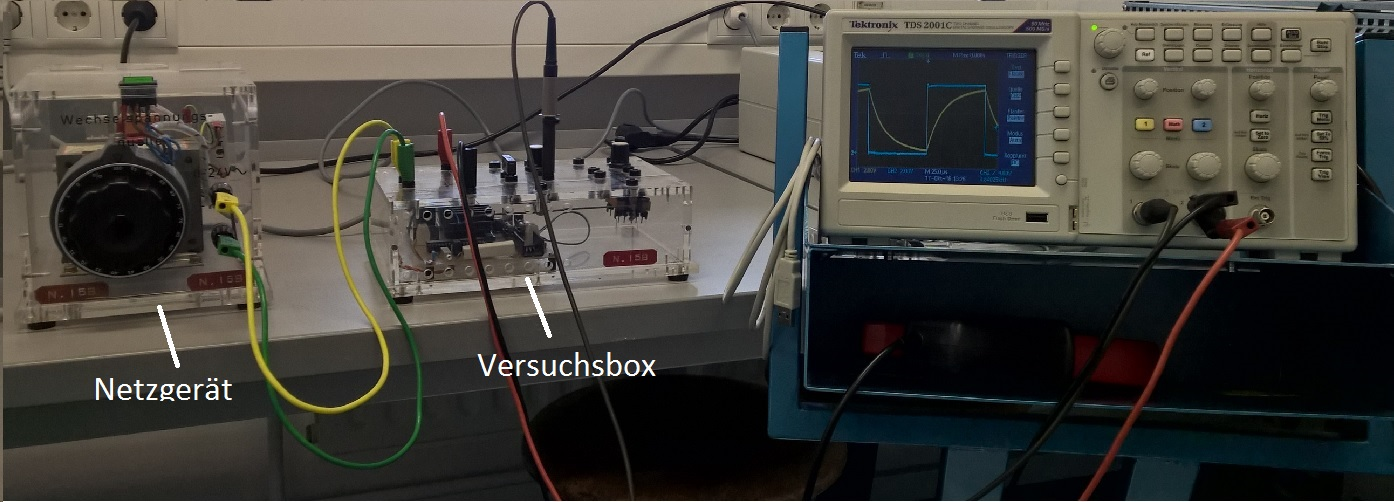
\includegraphics[width=0.9\textwidth]{Abbildungen/Aufbau_RC.jpg}
		\label{fig:Aufbau_RC}
		\caption{Aufbau zur Auf- und Entladung eines Kondensators.}
	\end{figure}
 %
 \item Messung der Kapazität eines Kondensators mit dem Oszilloskop:\\
	Verbinden Sie nun den Festwiderstand mit dem Kondensator. Bringen Sie die Aufladungskurve des Kondensators mit bestmöglicher Zeitauflösung auf den Bildschirm und messen Sie die Spannung am Kondensator als Funktion der Zeit. Speichern Sie dazu wieder ein entsprechendes Bild auf dem USB Stick, um es zuhause auszuwerten.\\
	
	%Legen Sie dazu eine Folie (liegt im Praktikum aus) über den Bildschirm und pausen sie den Kurvenverlauf ab. (Skalen und Einstellungen mit aufschreiben !!)\\
 	Ebenso nehmen Sie ein Bild der Entladung des Kondensators (dazu Triggerflanke (Trig Menu) ändern!) auf. Hätte man man sich durch geschicktes Drehen/Spiegeln der Aufnahme der Aufladekurve ggf. die Aufnahme der Entladekurve sparen können? Bitte begründen Sie Ihre Antwort.
 %
 \item Hochpass-Charakteristik des R-L-Kreises:\\
  Entfernen Sie die Leiterbrücke zwischen $R_C$ und dem Kondensator und verbinden stattdessen $R_L$ mit der Spule. Betrachten Sie den Verlauf der Spannung über der Spule und speichern Sie ein Bild davon ab. 
 %
\end{enumerate}

%------------------------------------------------
\section{Auswertung} 
%------------------------------------------------
\begin{hint}
	Bitte fertigen Sie die Graphen in der folgenden Auswertung per Hand auf Millimeterpapier an.
\end{hint}

\begin{enumerate}
 %
 \item Beschreiben Sie den Einfluss verschiedener Widerstände bei der Auf- und Entladung eines Kondensators über einen Widerstand (R-C-Kreis) anhand der Aufnahmen des Oszilloskops, die Sie gespeicherthaben. Beachten Sie dabei den Zusammenhang $\tau = R\,C$ und ggf. die Ladung auf dem Kondensator.
 %
 \item Bestimmung der Kapazität $C$ des Kondensators:
  \begin{enumerate}
   %
   \item Übertragen Sie den Kurvenverlauf der Aufladung des Kondensators auf Millimeterpapier. Einheiten und Achsenbeschriftung nicht vergessen!
   %
   \item Für die Aufladung eines Kondensators gilt:
    \begin{equation}
     U_C(t) = U_0\, \left(1-e^{-t/\tau}\right), \quad \tau = R\, C
    \end{equation}
		Lösen Sie diese Gleichung nach $e^{-t/\tau}$ auf und berechnen Sie den natürlichen Logarithmus. Schreiben Sie die neue Gleichung hin. Berechnen Sie die Unsicherheit des Logarithmus.
	 %
   \item Tragen Sie $\ln\left(1-U_C(t)/U_0\right)$ gegen $t$ auf. 
   %
   \item Bestimmen Sie aus der Steigung der Geraden die Kapazität $C$ des Kondensators inklusive Fehler. %Siehe hierzu Kapitel TODO: Kapitel über Fehler bei Geradensteigung/-achsenabschnitt!
   %
  \end{enumerate}
 %
 \item Erläutern Sie kurz, warum man einen R-L-Kreis auch Hochpass nennt.
 %
\end{enumerate}

\end{document}